% !Mode:: "Tex:UTF-8"
\chapter{绪论}
%命题可满足(简称SAT)问题求解是最古老也是最广泛使用的的计算引擎之一。许多电路设计和软件验证问题、密码求解问题均可转换为可满足性问题,并由SAT求解器求解。
%随着网格计算和云计算的发展,SAT求解也成为开放环境下最普遍的一种计算服务,科研机构、云计算服务公司都试图或已经推出了开放环境下基于SAT求解的验证和密码破解应用。
%同开放环境下的多数计算服务面临同样的困境,数据隐私问题一直是阻碍SAT计算在电路设计、软硬件验证和密码破解等重要应用中发挥作用的决定性因素。本文将对软硬件设计验证中SAT 问题进行研究,从实用性的角度出发,研究其中的数据隐私保护问题,以实现开放环境下可信SAT 求解。
%
%命题可满足性问题(SAT问题)是第一个被证明的NP完全问题,是一切NP 完全问题的“种子”,任何NP完全问题都可在多项式时间内转化为SAT 问题进行求解。当前SAT求解方法在测试向量自动生成、符号模型检查及组合等价性检查等电子设计自动化领域中得到了广泛的应用。可见,对SAT 问题的研究有着重要的理论意义和应用价值
%
%命题可满足性问题(简称SAT问题)\upcite{SATtheory}求解是最古老也是最广泛使用的的计算引擎之一。许多电路设计和软件验证问题、密码求解问题均可转换为可满足性问题,并由SAT求解器求解。
%随着网格计算和云计算的发展,SAT求解也成为开放环境下最普遍的一种计算服务,科研机构、云计算服务公司都试图或已经推出了开放环境下基于SAT求解的验证和密码破解应用。

随着云计算和网格计算等基于互联网的按需计算模式由概念走向实践,
基于互联网开放环境下的计算基础设施正逐渐成为计算资源和存储资源的主要提供方式之一。
%以Amazon EC2、Google App Engine 等为代表的云
%以IBM为代表的PAAS
%数据中心的增长
%Google Developers. What is BigQuery [EB/OL]. https://developers.
%google.com/bigquery/what-is-bigquery.
%根据艾默生的报告[17],目前全球云数据
%中心建设的规模已经接近百万个。
%而Gartner 公司预测2012 年至2017 年间,云数
%据中心的数量将以年均复合增长率4\%的速度增长[18]。
%17 Emerson Network Power. Emerson Network Power Sizes Up the State of the Data
%Center in 2011 [R]. 2011.
%18 Jonathon H. Forecast: Data Centers Worldwide 2010-2017 2Q13 Update [R]. 2013.
与此相适应,在开放计算环境下提供存储和计算服务,实现随时随地数据访问和按需计算,使用户摆脱地域束缚,也成为一种非常有吸引力的解决方案。

与此同时,
命题可满足性问题(SAT问题)是计算机科学和工程领域的一个重要问题。
SAT求解算法针对特定的命题逻辑公式,
搜寻对其变量集合的一个赋值,
以使该公式为真。
SAT 求解算法在测试向量自动生成、
符号模型检验及组合等价性检查等电子设计自动化领域\upcite{HardwareSAT},以及密码破解中得到了广泛的应用。
%引用
% 密码破解 Extending SAT Solvers to Cryptographic Problems. SAT 2009:
随着网格计算和云计算的发展,
SAT求解也成为开放环境下最普遍的计算服务之一。
科研机构、云计算服务公司都试图或已经推出了开放环境下基于SAT求解的验证和密码破解应用
\upcite{DBLP:conf/IEEEcloud/BrunM12,Nordugrid,DBLP:journals/concurrency/ChrabakhW07,OneSpin,CloudSMT}。。

但是,和存储服务的迅速普及不同,对计算隐私泄露的担忧一直阻碍着计算服务的商业化普及。
目前实用的加密技术,
如基于属性的加密技术\upcite{DBLP:journals/iacr/SahaiW04,DBLP:journals/iacr/GoyalPSW06,DBLP:conf/ccs/GoyalPSW06},
可以实现对加密数据的细粒度访问控制,从而解决数据传输或存储中的隐私保护,但却无法直接应用于计算数据。
可搜索存储加密技术\upcite{DBLP:journals/iacr/CurtmolaGKO06,DBLP:conf/ccs/CurtmolaGKO06,
DBLP:journals/jcs/CurtmolaGKO11}解决了开放环境下数据隐私性和可搜索性共存问题,但也仅仅适用于搜索计算。
全同态加密\upcite{DBLP:conf/stoc/Gentry09}从理论上提供了对通用计算透明的数据隐私性保护策略,
但其计算复杂性过高,仍不能满足实用性的要求。
类似的,
数据隐私问题一直是阻碍开放环境SAT求解在电路设计、软硬件验证和密码破解等重要应用中发挥作用的决定性因素。
本文将对软硬件设计验证中SAT 问题进行研究,
从实用性的角度出发,
研究其中的数据隐私保护问题,
以实现开放环境下可信且高效的SAT 求解。

%随着云计算、网格计算等基于互联网的按需计算模式由概念走向实践,开放环境下的计算基础设施正逐渐成为计算资源和存储资源的主要提供方式。
%与此相适应,在开放计算环境下提供存储和计算服务,实现随时随地数据访问和按需计算,使用户摆脱地域束缚,也成为一种非常有吸引力的解决方案。
%但是,和存储服务的迅速普及不同,对计算隐私泄露的担忧一直阻碍着计算服务的商业化普及。
%目前成熟的加密算法可以以较小的代价,解决数据传输或存储中的隐私保护,但却无法直接应用于计算数据。
%可存储加密技术、基于属性的加密技术从某些方面解决了开放环境下数据隐私性和可操作性的共存,
%但对通用计算透明的加密算法,其研究还方兴未艾。
\section {可满足问题}
\subsection{可满足问题以及相关概念}
在分析SAT求解问题的隐私保护之前,有必要对软硬件设计验证领域SAT 计算的相关概念进行介绍。
%%\subsection{可满足问题及其编码}
\subsubsection{可满足问题}
布尔集合表示为 $\mathbf{B}=\{0,1\}$。对于一个布尔变量集合$V$上的公式 $F$,
命题可满足问题(简称SAT问题)是指寻找一个可满足赋值$A : V\to \mathbf{B}$,使得 $F$为$1$。
如果这样的可满足赋值存在,$F$就是可满足的,可满足赋值称为公式$F$的一个解;
否则,$F$是不可满足的。公式的不可满足子集称为不可满足核。
搜索可满足赋值$A$的计算程序称为SAT求解器\upcite{Minisat}。

通常情况下,SAT求解器接受的输入公式是合取范式(CNF),
其中公式为子句的合取,
子句是文字的析取,而文字则是变量或是反。

公式(\ref{eqn_phi})的$\Phi$ 是一个CNF公式,
包含四个变量$x_1$, $x_2$, $x_3$, $x_4$和三个子句 $x_1\vee \neg x_2$, $x_2\vee x_3$, $x_2\vee \neg x_4$,
在子句$x_1\vee \neg x_2$ 中,文字$x_1$是变量$x_1$的正文字,
而文字$\neg x_2$是变量$x_2$ 的负文字。

\begin{equation}\label{eqn_phi}
\centering \Phi=(x_1\vee \neg x_2)
\wedge(x_2\vee x_3)
\wedge(x_2\vee \neg x_4)
\end{equation}

%The number of literals in clause $C$ is denoted as $|C|$.
%The number of clauses in a CNF formula $F_C$ is denoted as $|F_C|$。
%For example $| x_1\vee  \neg x_2 |\equiv 2$,
%while $|\Phi|\equiv 3$.
子句$C$中文字的数量记为$|C|$。
CNF公式$F$中的子句数记为$|F|$。
例如$| x_1\vee  \neg x_2 |\equiv 2$,而$|\Phi|\equiv 3$。

%Variable set of CNF formula $F_C$ is denoted as $V_{F_C}$.
CNF公式$F$的变量集合,记为$V_{F}$。
%When variables in CNF formula $F_C$ are assigned with solution $S_C$, we denote it as $F_C(S_C/V_{F_C})$.
CNF公式$F$中所有变量被赋值为解$A$,
记为$F(A/V_{F})$。
% \begin{definition}[$V_{F}$]\label{VariableSet}
% $V_{F}$ denotes variable set of CNF formula $F$.
% \end{definition}

% \begin{definition}[$F(S/V_{F})$]\label{VariableAssignment}
% Variables in CNF formula $F$ are assigned with $S$, denoted as $F(S/V_F)$,
% \end{definition}
%\subsubsection{Tseitin编码}

%In hardware verification,
%circuits and properties are converted into CNF formula by Tseitin encoding\upcite{Tseitin},
%and then CNF formula is solved by SAT solver.
%Circuits can all be expressed by a combination of gate AND2 and INV,
%so we only list Tseitin encoding of gate AND2 and INV here.
\subsubsection{Tseitin编码}\label{subsubsec_tseitin}
在硬件验证过程中,
电路和属性通过Tseitin编码\upcite{Tseitin}转换为CNF公式,
而后交给SAT求解器求解。
由于所有电路都可以被表示为二输入与门AND2和非门INV的组合形式,
所以在这里我们仅仅给出AND2门和INV门的Tseitin编码:

\begin{enumerate}
\item 对于非门 $z=\neg x$,
由Tseitin编码产生的CNF公式为$(x\vee z)\wedge( \neg x\vee \neg z)$。
\item 对于二输入与门 $z=x_1\wedge x_2$,
由Tseitin编码产生的CNF公式为$( \neg x_1\vee \neg x_2\vee z)\wedge(x_1\vee \neg z) \wedge(x_2\vee \neg z)$。
\item 对于一个表示为二输入与门和非门组合的复杂电路$C$,
由Tseitin编码产生的CNF公式$Tseitin(C)$ 是所有这些门的Tseitin 编码的合取。
\end{enumerate}

对于一个包含非门$d=\neg a$和二输入与门$e=d\wedge c$的简单电路$C$,
由Tseitin编码产生的CNF公式如公式(\ref{eqn_andinv})所示。


\begin{multline}\label{eqn_andinv}
% \begin{equation}\label{eqn_andinv}
Tseitin(C)=
\left\{
\begin{array}{cc}
& (a\vee d) \\
\wedge & (\neg a\vee \neg d)
\end{array}
\right\}\wedge\left\{
\begin{array}{cc}
& (\neg e\vee c) \\
\wedge & (\neg e\vee d) \\
\wedge & (e\vee \neg c\vee\neg d)
\end{array}
\right\}
% \end{equation}
\end{multline}


\subsection{可满足问题求解}

\subsubsection{可满足问题的简单解法}
为了方便对SAT求解过程的描述,我们以图\ref{basic_circuit}中的电路为例子,首先给出一个简单低效但是直观的求解方法。并在下面逐步描述对该方法的改进措施,从而最终描述清楚现代SAT求解器中常用的高效算法。

\begin{figure}[t] % use float package if you want it here
  \centering
  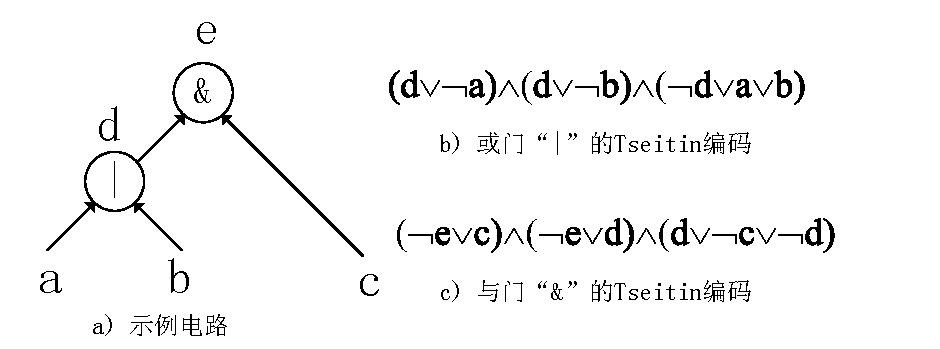
\includegraphics[width=0.8\textwidth]{fig_basic_circuit}
  \caption{示例电路及其编码}
  \label{basic_circuit}
\end{figure}


最简单的SAT求解算法是简单地遍历所有可能的变量赋值,形成树形的二叉搜索空间。对于图\ref{basic_circuit}b)的SAT公式,将导致图\ref{basic_search}所示的二叉搜索树。其中打钩的叶节点表示合法的求解结果。每次对特定变量进行二叉分解的步骤称为决策,每次决策产生一个新的决策层。图\ref{basic_search}的决策层1、2和3分别对应于分别对变量a、b和c进行二叉分解。

\begin{figure}[b] % use float package if you want it here
  \centering
  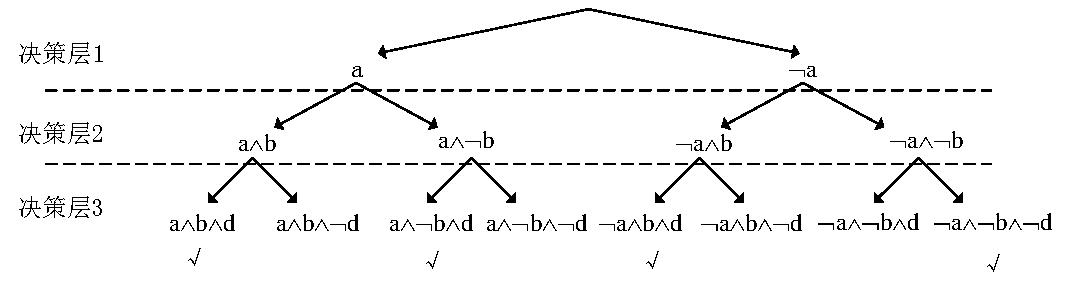
\includegraphics[width=0.8\textwidth]{fig_basic_search}
  \caption{基于完全二叉树遍历的SAT求解}
  \label{basic_search}
\end{figure}

\subsubsection{布尔约束传播(BCP)}
为了使一个特定的SAT公式成立,必须使其中每个子句都成立。
而为了使某个特定子句成立,其中必须存在至少一个文字成立。
因此当在某个子句中,只有一个特定的文字$w$尚未取值,而其他所有文字均取值为$0$时,
则该文字必须取值为$1$。
如果该文字为某个特定变量$v$,这将导致$v$取值为$1$,否则取值为$0$。
这一推导过程称为布尔约束传播。

以图\ref{basic_circuit}b)的或门的Tseitin编码为例,
为了使该公式成立,每个子句都必须成立。
以第一个子句$d \wedge a$为例,当$a$ 为$1$时,
$d \wedge a$化简为$d$,
为了使其成立,$d$必须取值为1。
此时搜索树如图\ref{BCP} 所示。
其中粗线代表在特定决策层内部的BCP 操作。

\begin{figure}[t] % use float package if you want it here
  \centering
  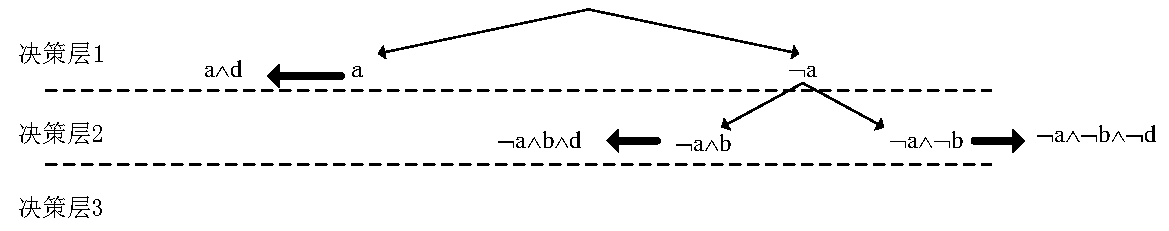
\includegraphics[width=0.8\textwidth]{布尔约束传播}
  \caption{布尔约束传播}
  \label{BCP}
\end{figure}

\subsubsection{冲突指导的子句学习}
冲突指导的子句学习和非正交回溯\upcite{DBLP:conf/iccad/ZhangM02} 是提升SAT求解器性能的另一个重要手段。其中非正交回溯与与本文重点关注的数据结构关系不大,因此将仅描述冲突指导的子句学习。

为了简明起见,仍然使用一个例子描述冲突指导的子句学习。如图\ref{confict}所示的一个二叉搜索树,当到达红色的标记为conflict 的节点时,有$\{a \equiv 0,b \equiv 0, c \equiv 0,d \equiv1,e \equiv 0,f \equiv1\}$。这将导致某个短句中的所有文字均成为0,称这种情况为一个冲突(conflict)。 此时冲突分析算法将对该子句中的每一个文字,沿着如图\ref{confict}粗线所示的BCP 关系逆向回溯,以便找到导致此次冲突的根本原因。假设找到的三个变量分别为$\{c \equiv 0,d \equiv 1,f \equiv 1\}$,这意味着a、b和e与本次冲突无关。无论以后a、b 和e 取任何值,只要遇到$\{c \equiv 0,d \equiv 1,f \equiv 1\}$ 的情况,都不必继续搜索。这意味图\ref{confict}中绿色所示的分支都可以被剪掉。

为了达到这种剪枝效果,将对冲突分析的结果中每个变量取反,以构造一个冲突学习子句。即$\{c \equiv 0, d \equiv 1, f \equiv 1\}$ 将会产生一个冲突学习子句$\{c\vee \neg d \vee \neg f\}$,并加入子句数组。以后每次当c、d和f三个变量中的两个满足$\{c \equiv 0, d \equiv 1, f \equiv 1\}$,则将立即通过冲突学习子句产生一次BCP,使得第三个变量无法满足$\{c \equiv 0,d \equiv 1,f \equiv 1\}$。 这就构成了一次剪枝操作。

\begin{figure}[t] % use float package if you want it here
  \centering
  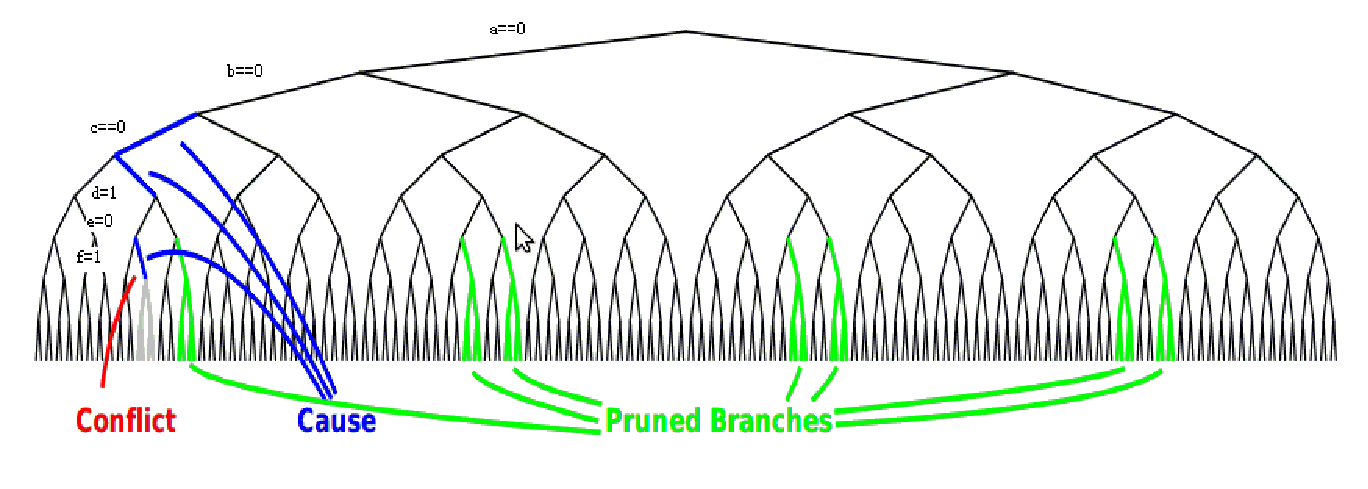
\includegraphics[width=0.8\textwidth]{fig_conflict}
  \caption{冲突指导的子句学习}
  \label{confict}
\end{figure}


\subsubsection{MiniSat 求解器的递增求解机制}\label{subsec_incsat}

本文中,
我们使用MiniSat 求解器\upcite{EXTSAT} 求解所有CNF公式。
和其他基于冲突学习机制\upcite{CONFLICTLEARN}的SAT求解器类似,
MiniSat 从在搜索中遇到的冲突中产生学习短句,
并记录他们以避免类似的冲突再次出现。
该机制能够极大的提升SAT求解器的性能。

在许多应用中,
经常存在一系列紧密关联的CNF公式。
如果在一个CNF公式求解过程中得到的学习短句能够被其他CNF公式共享,
则所有CNF公式的求解速度都能够得到极大的提升。

MiniSat 提供了一个增量求解机制以共享这些学习短句。
该机制包括两个接口函数:
\begin{enumerate}
\item
$addClause(F)$ 用于将一个CNF公式$F$ 添加到MiniSat的短句数据库,
以用于下一轮求解。
\item
$solve(A)$ 接收一个文字集合$A$作为假设,
并求解CNF 公式$F\wedge \bigwedge_{a\in A} a$。
其中$F$是在$addClause$中被加入短句数据库的CNF公式。
\end{enumerate}

基于该机制,
可以针对一个相同的CNF公式$F$,
使用不同的文字集合$A$,
来产生并递增地高效求解不同的$F\wedge \bigwedge_{a\in A} a$。


\subsection{可满足赋值遍历}\label{subsec_relallsat}
多数时候,可以满足特定SAT问题的解并不是唯一的,
求出所有可满足解的过程被称为可满足赋值遍历(简称ALLSAT求解)。

ALLSAT求解由基于SAT求解的可满足赋值遍历算法来实现。
直观上看,调用一次SAT求解器可以获得SAT问题的一个解,也就是一个完整的可满足赋值。
将这个完整的可满足赋值中每一个文字取反,构造出阻断(block)子句并加入到待求解的SAT问题公式中,
以引导SAT求解器避开已搜索过的解。
通过多次重复,最终可以获得SAT问题所有的解。

绝大多数可满足赋值遍历算法致力于将由SAT求解得到的一个完整的赋值扩展为一个包含较多赋值的赋值集合,
以便减少调用SAT求解器的次数并压缩存储赋值解的空间开销。
文献\upcite{SATUNBMC}提出了第一个此类算法。
他在SAT求解器求解过程中构造一个蕴含图,
用以记录每个赋值之间的依赖关系。
每个不在该图中的赋值变量都可以从最终结果中剔除。
在文献\upcite{MINASS} 和\upcite{REPARAM}中,
每个变量如果在其不被约束的情况下不能使$obj\equiv 0$ 被满足的话,
则该变量可以从最终结果中剔除。
在文献\upcite{MINCEX} 和\upcite{PRIMECLAUSE,EFFCON}中,
冲突分析方法被用于剔除与可满足性无关的变量。
在文献\upcite{MEMEFFALLSAT}中,
变量集合被划分为重要变量和非重要变量集合。
搜索过程中重要变量的优先级高于非重要变量。
因此重要变量子集构成了一个搜索树,
而该树的每一个叶节点是非重要变量的一个搜索子树。
%Tobias Nopper et al.\upcite{CMPMINCEX} propose an counterexample minimization algorithm for incomplete designs that contain black box.
Cofactoring \upcite{EFFSATUSMCCO} 则通过将非重要变量设置为SAT求解器返回的值以缩减搜索空间。

另一类算法通过Craig插值以扩大解集合。
文献\upcite{InterpBoolFunction}提出了第一个此类算法。
该算法构造两个相互矛盾的公式,并从他们的不可满足证明中抽取Craig 插值。
在文献\upcite{interpNoProof}中,
Craig插值的产生过程类似于传统的可满足赋值遍历算法。
不过其扩展算法包含两步,
分别对应于两个参与计算的公式。
该算法是第一个不需要产生不可满足证明的Craig插值算法。

\subsection{Craig插值的原理和实现}\label{sec_craigimp}
在通常的SAT求解器,
包括本文使用的MiniSat\upcite{EXTSAT}中,
要求待求解的公式被表示为CNF格式。
其中一个公式是多个子句的合取(conjunction),
而每一个子句是多个文字的析取(disjunction),
而每个文字是一个布尔变量$v$或者其反$\neg v$。
如公式$(v_0\vee\neg v_1\vee v_2)\wedge(v_1\vee v_2)\wedge(\neg v_0\vee v_2)$,
包含子句$v_0\vee\neg v_1\vee v_2$,$v_1\vee v_2$和$\neg v_0\vee v_2$。
而子句$v_0\vee\neg v_1\vee v_2$包含文字$v_0$, $\neg v_1$和$v_2$。

当存在一个变量$v$,
使得一个子句$c$中同时包含两个文字$v$和$\neg v$,
则称$c$为tautological的。
我们通常假设有待SAT求解器求解的公式中所有的子句都是非tautological的。

假设公式$F$的布尔变量全集为$V$。
若存在对$V$的赋值函数$A:V\to \{0,1\}$,
使得$F$中的每个子句均能取值为1,
则称$F$是可满足的,
此时SAT求解器能够找到赋值函数$A$。
否则称$F$为不可满足的,
此时SAT求解器能够产生如下一小节所述的不可满足证明。

\subsubsection{不可满足证明}
对于两个子句$c_1=v\vee A$和$c_2=\neg v\vee B$,
当$A\vee B$是tautological时,
$A\vee B$称为它们的\textbf{resolvant}。
而$v$称为它们的\textbf{pivot}。
易知以下事实:

\begin{equation}
\begin{array}{ccc}
&resolvant(c_1,c_2) = \exists v, c_1\wedge c_2 &\\
&c_1\wedge c_2 \to resolvant(c_1,c_2)&
\end{array}
\end{equation}

\begin{definition}
对于不可满足公式$F$,
假设其子句集合为$C$,
则其不可满足证明$\Pi$是一个有向无环图$(V_{\Pi},E_{\Pi})$,
其中$V_{\Pi}$是子句集合,
而$E_{\Pi}$是连接$V_{\Pi}$中子句的有向边集合。
$\Pi$满足如下要求:
\begin{enumerate}
\item 对于节点$c\in V_{\Pi}$:
  \begin{enumerate}
    \item 要么$c\in C$,此时称$c$为$\Pi$的根
    \item 或者$c$有且仅有两个扇入边$c_1\to c$和$c_2\to c$,
    使得$c$是$c_1$和$c_2$的resolvant。
  \end{enumerate}
\item 空子句是$\Pi$的唯一一个叶节点。
\end{enumerate}
\end{definition}

直观的说,
$\Pi$就是一棵树,
以子句集合$C$的子集为根,
以空子句为唯一叶节点。
而每个节点$c$的两个扇入边$c_1\to c$和$c_2\to c$代表了一个resolving关系$c:=resolvant(c_1,c_2)$。

包括本文使用的MiniSat求解器\upcite{EXTSAT}在内的许多SAT求解器,
当公式不可满足时都将产生一个不可满足证明$\Pi$。

\subsubsection{Craig插值算法}

根据文献\upcite{Craig},
给定两个布尔逻辑公式$A$ 和$B$,
若$A\wedge B$ 不可满足,
则存在仅使用了$A$ 和$B$共同变量的公式$I$ ,
使得$A\Rightarrow I$且
$I\wedge B$不可满足。
$I$ 被称为$A$针对$B$的Craig插值\upcite{Craig}。

目前最常见且最高效的产生Craig插值的算法是
McMillan算法\upcite{interp_McMillan} 。
其基本原理描述如下。

对于上述公式$A$和$B$,
已知$A\wedge B$不可满足,
而$\Pi$是SAT求解器给出的不可满足证明。
当一个变量$v$同时出现在$A$和$B$中时,
我们称其为全局变量。
若$v$只出现在$A$中,
则称其为$A$本地变量。

对于文字$v$或者$\neg v$,
当变量$v$是全局变量或者$A$本地变量时,
称该文字为全局文字或者$A$本地文字。

对于子句$c$,
令$g(c)$为$c$中所有全局文字的析取,
而$l(c)$为$c$中所有$A$本地文字的析取。

例如,
假设有两个子句$c_1=(a\vee b\vee\neg c)$ 和
$c_2=(b\vee c\vee\neg d)$。
并假设$A=\{c_1\}$和$B=\{c_2\}$。
则$g(c_1)=(b\vee\neg c)$,
$l(c_1)=(a)$,
$g(c_2)=(b\vee c)$,
$l(c_2)=FALSE$。


\begin{definition}\label{def_gencraig}
令$(A,B)$为一对公式,
而$\Pi$是$A\wedge B$的不可满足证明,
且其唯一叶节点是空子句$FALSE$。
对于每一个节点$c\in V_{\Pi}$,
令$p(c)$为如下定义的一个公式:
\begin{enumerate}
\item 如果$c$是根节点则
  \begin{enumerate}
    \item 如果$c\in A$则$p(c)=g(c)$
    \item 否则$p(c)=TRUE$
  \end{enumerate}
\item 否则令$c_1$和$c_2$分别是$c$的两个扇入节点,而$v$是他们的pivot变量
  \begin{enumerate}
    \item 如果$v$是$A$本地变量,则$p(c)=p(c_1)\vee p(c_2)$。
    \item 否则$p(c)=p(c_1)\wedge p(c_2)$。
  \end{enumerate}
\end{enumerate}
\end{definition}

上述定义\ref{def_gencraig}是构造性的,
已经给出了从不可满足证明$\Pi$得到最终的Craig插值的算法,
即以$\Pi$的根节点为起点,
为每一个$c$计算相应的$p(c)$,
直至到达最终的唯一叶节点$FALSE$。
我们有以下定理:

\begin{theorem}
定义\ref{def_gencraig}为唯一叶节点$FALSE$产生的$p(FALSE)$即为
$A$相对于$B$的Craig插值。
\end{theorem}

该定理的详细证明可见文献\upcite{DBLP:journals/tcs/McMillan05}。

计算$A$相对于$B$的Craig插值的时间复杂性为$O(N+L)$,
其中$N$是$\Pi$中包含的节点个数$|V_{\Pi}|$,
而$L$是$\Pi$中的文字个数$\Sigma _{c\in V_{\Pi}}|c|$。
而所产生的插值可以视为一个电路,
其空间复杂性为$|O(N+L)|$。
当然,
$\Pi$的尺寸在最坏情况下也是$A\wedge B$的尺寸的指数。

%\subsection{对偶综合}\label{subsec_relallsat}


\section{面向软硬件设计验证的可满足问题求解}
可满足问题(SAT)\upcite{SATtheory}是硬件电路设计和软件可信验证领域\upcite{HardwareSAT,softwareSAT} 共同关注的重要问题。许多重要的电路设计和软件验证问题均可转换为可满足性问题,并由SAT求解器求解。随着集成电路制造工艺的发展,在单个芯片内集成的晶体管个数将在2020年接近一千亿;而社会信息化程度的提高促使软件系统越来越复杂,以Linux操作系统为例,在2008 年仅其内核代码就已经突破1千万行。软硬件系统的规模日益增大,服务于硬件设计和软件验证的SAT求解器的运算量也急剧攀升。在过去的10年,作为形式化工具基本引擎的SAT 求解器性能已经显著提升,几分钟内即可处理数百万变量和数亿子句,但是依然无法满足日益增长的计算要求。

传统的硬件辅助与设计(EDA)综合与验证工具的核心框架通常包含以下主要功能模块:

1.抽象问题表示:该模块用于管理与特定推理过程和引擎无关,但是与问题本身密切相关的数据结构,如简化布尔电路(Reduced Boolean circuits)\upcite{DBLP:conf/tacas/AbdullaBE00}和
与非图(And-Inverter Graph)\upcite{Brummayer06localtwo-level}等。

2.问题编码:该模块用于将特定的抽象问题表示,转换为满足特定推理引擎,
如二叉决策图(简称BDD)\upcite{DBLP:journals/tc/Bryant86} 或SAT要求的数据结构,以便进行高效的推理工作。针对SAT推理引擎,该模块通常使用在空间和时间方面均具有多项式复杂性的Tseitin\upcite{Tseitin} 编码。

3.BDD和SAT推理引擎:这两个模块负责具体的推理工作。
绝大多数EDA工具和软件验证工具的核心推理引擎为二叉决策图(BDD)和可满足求解器(SAT)。其中BDD受到归一化表示方式导致的状态空间爆炸问题的困扰,通常仅用于需要归一化特性的小规模推理问题,如抽象谓词的表示等。而SAT则通常较少受到状态空间爆炸的影响,且天生具有内在的并行性和可扩展性;另一方面SAT问题是NP难问题,其求解时间和问题结构相关,对计算资源的需求也随具体问题而不同。

软件程序验证工具也具有类似于硬件设计验证工具的核心框架。
SAT求解器通常是作为核心推理引擎集成到具体问题求解器中。
因此,从逻辑流程上看,
硬件和软件形式化验证通常都是通过抽象问题表示之后再进行问题编码,
而后将问题的可满足性求解过程交给SAT 求解器完成,
流程如图\ref{verfication-procedure}所示。

\begin{figure}[t] % use float package if you want it here
  \centering
  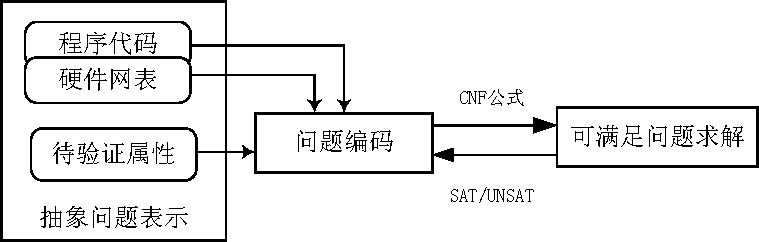
\includegraphics[width=0.8\textwidth]{验证流程}
  \caption{基于SAT求解的软硬件验证流程}
  \label{verfication-procedure}
\end{figure}

因此将软硬件设计验证中产生的复杂SAT 问题外包到云或网格环境下,利用其提供的弹性计算资源,成为一种有吸引的解决方案。
科研机构和商业公司也已经开展了在云和网格环境下进行SAT问题求解的研究
\upcite{DBLP:conf/IEEEcloud/BrunM12,Nordugrid,DBLP:journals/concurrency/ChrabakhW07,OneSpin,CloudSMT}。
如美国华盛顿大学研究小组推出支持云SAT求解的sTile系统\upcite{DBLP:conf/IEEEcloud/BrunM12};
芬兰阿尔托大学研究小组推出基于NorduGrid的SAT求解器\upcite{Nordugrid};
美国圣巴巴拉大学研究小组推出GridSAT系统\upcite{DBLP:journals/concurrency/ChrabakhW07};
形式化验证服务提供商OneSpin 公司和Plunify公司于2013年,
联合推出了面向云平台的基于SAT求解的硬件验证商业服务\upcite{OneSpin}。

\section{开放环境下数据隐私的安全威胁}
云计算和网格依托于互联网,与互联网这种开放环境的便利快捷相伴而生的是,安全威胁也无处不在。
一方面,公有云和网格计算节点均直接部署在广域网上,与用户处于不同的安全域。
用户的服务请求可能面临来自网络中的多重威胁;
另一方面,云服务提供商或是网格计算节点无法证明其内部行为可以信任。

由于网格计算是由松散耦合的高端计算设施组成\upcite{Nordugrid},网格环境下恶意计算节点是客观存在的\upcite{HV-grid};
而在云计算环境下,虽然云硬件平台提供商及其基础设施(虚拟层)是可被信赖,在其上运行的虚拟机却不总是可以信赖的。
文献\upcite{AMI}指出,著名的云计算提供商亚马逊的EC2受到了虚拟机影像滥用的困扰,被污染虚拟机映像会迅速扩散到整个社区;
而文献\upcite{InformationLeakageofCloud} 则指出了处于同一台物理机器上的虚拟机之间攻击的可能性。
与此相照应,早在2007年,
《华盛顿邮报》就披露了客户关系管理领域著名的云服务提供商Saleforce.com由于受到安全攻击而导致大量租户数据泄露与丢失\upcite{washingtonPostSaleForce};
2010 年下半年谷歌解雇了两名入侵租户的私有账户以获取隐私数据的员工\upcite{googelFiresTwoEmployees}。
Gartner 公司发布的研究报告\upcite{gartner70}显示,所采访的企业中70\%以上认为出于对数据安全性与隐私保护的怀疑,
在近期内不会采用云计算技术。
RSA 首席技术官也指出\upcite{rsaSafe},在企业将现有的应用向第三方云服务提供商提供的云环境迁移过程中,
要考虑的首要问题是对云计算的数据安全问题。
此处的安全不仅指数据的可用,更加注重的是数据的隐私保护。
针对OneSpin公司推出的硬件形式化验证云服务,新闻评论\upcite{oneSpinsafe}指出验证数据的隐私是用户最为关心的因素。

而针对计算结果的安全性,对早期的志愿计算SETI@home项目的统计发现\upcite{HV-grid},这类基于网格的开放计算环境存在三类威胁:
\textbf{私心的计算参与者}:由于计算结果具有稀缺性,私心的计算参与者会出现奇货可居的意识,他们会完全遵照协议的规定,尽力计算出正确结果,但会出于利益原因,将有价值的结果信息透露给第三方,从而损害用户的隐私安全。
\textbf{懒惰的计算参与者}:由于大计算量会耗费很多计算资源,出于节约计算成本的考虑,计算参与者可能不按照约定来进行足量的计算,以此来节省开销,使用部分结果来作为最终结果。
\textbf{恶意的计算参与者}:可能出于某种目的,计算参与者完全违反协议规定,随意返回错误结果来欺骗用户,误导用户决策。
而在2009年对云计算模型和网格计算模型的比较一文\upcite{DBLP:journals/corr/abs-0901-0131} 中,Ian Foster 指出云计算在安全措施设计成熟度还远不及网格,这就使得网格计算下影响结果正确性的威胁也很可能对云计算环境造成影响。

这些事实指出,外包到云计算或网格这类开放环境下的SAT问题,
由于计算模式将数据和处理的控制权从用户转移至云服务方,导致具体的处理过程用户不可控;
其输入和输出数据可能会被未授权的第三方访问,
这些潜在的威胁者可能会从这些数据中获取有价值的信息。
糟糕的是,即使发生了上述信息泄露的情况,如果不辅助以技术手段,用户难以察觉和追踪;
更为恶劣的情况是,部署在网格或云环境下的SAT求解器可能会被迫使返回错误的结果。

来源于软硬件验证的SAT问题,可能遭受硬件结构信息泄露的问题;Roy\upcite{csRoy} 和Fu\upcite{csFu}的工作指出了从CNF 公式中抽取电路结构信息的可能性。Zvika\upcite{OBfuscationd-CNFs}、Yuriy Brun\upcite{DBLP:conf/IEEEcloud/BrunM12} 等人的工作也指出在云计算环境下进行SAT问题求解需要解决隐私保护问题。另一方面,Du\upcite{HV-grid} 将某些复杂SAT问题的解称作高价值稀有事件,指出SAT问题的解也应该被视作为隐私;如来源于密码破解的SAT问题,奇货可居的计算参与者可能会因利益问题而将其泄露给第三方。

\section{开放计算环境下可满足问题求解的隐私保护问题}
开放环境下的这些威胁将SAT计算服务的潜在用户置于进退维谷的境地:
使用公共的云计算或网格计算基础设施在系统维护性和可用性上面具有较高的性价比,
但却会面临隐私泄露和错误结果等安全问题的困扰。
在开放计算环境下,计算数据的隐私保护问题看起来是一个不可能完成的问题:由于计算是在开放环境下完成的,未经加密处理的原始输入和输出数据势必会引发泄露的风险,而经过传统加密算法处理之后的计算数据由于对计算不再透明,因而丧失了可计算性。因此在保持可计算性的前提下,讨论SAT数据的隐私保护,成为了开放计算环境下的最大挑战。

2009 年,Gentry 等人针对开放计算环境下的数据隐私保护问题,提出完全同态加密的概念。
这一概念描绘了开放环境下计算外包的美好愿景:经过完全同态加密,在保持数据隐私性的同时,仍然可保持原有数据的可计算性。完全同态加密的理论基础是,由于任何计算都可以分解为一系列微观加乘计算,并且在有限步内对加乘计算透明的加密算法确实存在。
因而任意的计算都可以分解为一系列的有限次针对加密数据的加乘计算。
这无疑从理论上扫清了开放环境下计算外包的安全障碍。但是,由于完全同态加密需要将计算分解为细粒度的有限步加乘计算。
所带来的昂贵计算开销,使其距离实用化还有相当的距离。

同样为了解决外包计算的数据隐私保护,Atallah等提出了针对具体问题,进行计算数据伪装的概念。例如针对矩阵求解类计算,将有待外包的数据与随机对角矩阵进行矩阵乘,对外包的矩阵数据进行伪装加密。
由于矩阵计算的可逆性,伪装加密后结果可以通过可逆的矩阵运算得到。数据伪装方法充分利用了问题的特点,不改变原有计算过程和数据的外在形式,是一种直接实用的方案。但目前针对SAT 问题的数据伪装的研究还处于空白。

作为一种基础的计算引擎,软硬件设计问题中的SAT问题具有其内在的特点:任何硬件设计和软件程序都可以表示为与或非等门的集合。
本文从实用化的角度出发,希望在复用原有求解器的前提下,探讨软硬件设计、验证领域中SAT 问题的隐私保护方法。

\subsection{CNF公式中的结构信息}\label{CNF structure}
%\textbf{Circuit structure in CNF formula}\label{CNF structure}
%Since we want to protect circuit structure in CNF formula,
%let's first study how the circuit can be recovered from CNF formula.
%Literatures\upcite{csRoy,csFu} have proposed algorithms to recover circuit structure from CNF formula in details.
%Before discussing them, some concepts should be introduced first.
CNF公式是SAT求解的输入数据,来源于软硬件验证及设计中的CNF公式中会包含硬件电路结构信息;
文献\upcite{csRoy,csFu}给出了从CNF公式中获取电路结构信息的算法细节,首先了解算法中用到的概念。
%
%\begin{definition}[CNF signature]
%CNF signature of gate $g$ is its Tseitin encoding $Tseitin(g)$.
%Each clause in CNF signature is called characteristic clause.
%A characteristic clause containing all variables in CNF signature is a \textbf{key clause}.
%Variable corresponding to output of a gate is called \textbf{output variable}.
%\end{definition}
\begin{definition}[CNF标记]
门$g$的CNF标记就是它的Tseitin编码$Tseitin(g)$。
CNF标记中的每个子句称为门的\textbf{特征子句}。
包含门中所有变量的特征子句称为\textbf{关键子句}。
对应于门输出的变量称为\textbf{输出变量}。
\end{definition}

公式(\ref{eqn_andinv})中的 AND2门,
$\neg e\vee c$ 是它的一个特征子句,
$e\vee \neg c\vee\neg d$是它的关键子句。
$e$是输出变量。

文献\upcite{csRoy}指出,
在一种编码规则下,具有相同特征函数的门必然会被编码成为相同的CNF 标记,也就是相同的子句集合。
通过探索这种结构特征可以恢复电路结构,已知的结构检测算法基于以下定义的有向超图和二分图概念。

\begin{definition}[超图]\label{Hypergraph}
 以CNF公式中的子句为节点、变量为边,形成的图称为超图(Hypergraph)。
 超图$G(V,E)$ 中:
 $V$中每个节点对应$F$中一个子句;
 $E$中每条边对应$F$中一个变量。
 如果两个子句包含相同的变量,就在两个子句之间连接一条边,并用变量标注。
\end{definition}

在超图表示方式下,存在具有不同CNF标记的两个门,却具有相同超图表示的情况,
如AND3和OR3,均对应图\ref{graph}a)中的超图。
为了克服该问题,在电路结构检测算法\upcite{csRoy}中,使用有向超图进行区分。

\begin{definition}[有向超图]
在定义\ref{Hypergraph}给出的超图基础上,
根据子句中文字的正负、为边添加标记,
形成的图称为有向超图(Directed Hypergraph)。
\end{definition}

\begin{definition}[二分图]
将子句和变量均视为节点,同时将变量和子句的从属关系视为边,形成的图称为二分图(Bipartite Graph)。
在二分图$G(V,E)$中:
$V$中每个顶点对应于集合中的一个子句或一个变量,即$V=V_{cls}\bigcap V_{var}$,其中$V_{cls}$为子句集合、$V_{var}$ 为变量集合。
$E$中的每条边对应于一个子句/变量对,
如果变量出现在子句中,就在变量和子句之间连接一条边;变量为负值则对应一条负边,反之为正边。
\end{definition}

以AND门为例,AND3门的超图如图\ref{graph}a)所示;
其有向超图对应于图\ref{graph}b),其中使用$\uparrow$表示正,┼ 表示负;
其二分图对应于图\ref{graph}c) 所示的二分图。
\begin{figure}[t]
  \centering
  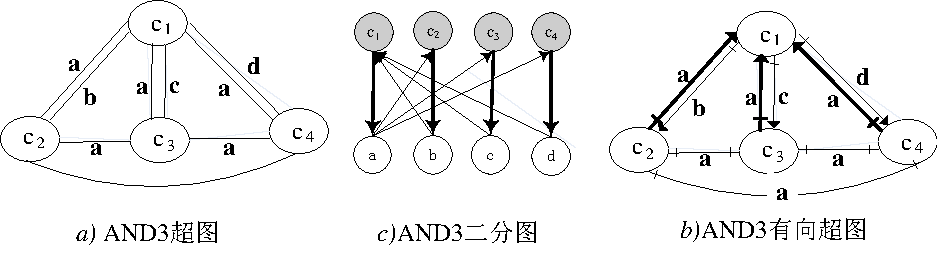
\includegraphics[width=0.8\textwidth]{超图二分图}
  \caption{超图和二分图}
  \label{graph}
\end{figure}

基于上述定义,CNF公式可以表示为包含多种CNF特征子图的超图或二分图。
这种图结构使得利用基于子图同构和模式匹配技术来恢复出电路结构和程序结构信息成为可能。

\subsection{SAT问题隐私保护的对象}
基于上述概念,
CNF公式可以转化超图$G$,
在图中匹配常用的CNF标记,通过同构子图的方式即可恢复出CNF公式携带的门信息。
进一步,可用最大无关集来表示恢复出来的电路信息。
基于关键子句和CNF标记的模式匹配还可以检测出所有门,并构建最大匹配门的子集。
除了门的结构信息,在来源于软硬件验证的CNF公式还包含了状态迁移关系。
Roy\upcite{csRoy}和Fu\upcite{csFu} 给出了具体的实现技术。
潜在的攻击者可以利用这些技术手段恢复出电路结构,并得到电路的状态迁移关系。
因此,CNF标记和关键子句是特别需要保护的重要信息。

另一方面,在验证领域,某些SAT问题的解反映了该系统的某些特性是否达到,因此解也应作为隐私加以保护。

\section{本文的主要工作}
来源于软硬件验证和设计的SAT 问题,
由于其CNF公式和其解中包含了电路结构以及电路迁移关系等敏感信息,在开放计算环境下求解,必须防止这些敏感信息的泄露。
本文的工作也围绕着保护上述敏感信息展开。

\subsection{已有工作的局限}
针对开放计算环境下的计算数据隐私保护问题,2009年Gentry\upcite{DBLP:conf/stoc/Gentry09} 等人开创性提出完全同态加密的概念。
经过完全同态加密,在保持数据隐私性的同时,仍然可保持原有数据的可计算性。由于任何的计算都可以分解为一系列微观加乘计算,因此寻找可保持对加乘的加密算法成为了一个努力的方向。
但是由于计算需要被分解为细粒度的有限步的加乘操作,因此同态加密后的计算效率一直制约着该方法的实用化。

针对CNF公式隐私保护方面相关的研究才刚刚开始,2013年Brakerski\upcite{OBfuscationd-CNFs} 等人面向云计算环境,首次探讨了使用多线性映射和坡度编码策略对d-CNF进行混淆的方法。
使用随机和带有噪声的编码,并提供测试过程来确保编码元素的等价。
这种方法基于有限加速假设,混淆后的CNF使用最原始的二叉树搜索的方法进行求解,无法利用目前经典的SAT求解器。

Yuriy Brun\upcite{DBLP:conf/IEEEcloud/BrunM12} 等人则使用了stile数据分布的模式,通过将数据条块计算,提高攻击者获得完整CNF 公式难度,以此降低数据被窃取的可能性。
该方法目前也仅仅支持简单的二叉遍历赋值求解方法,无法利用已有的SAT 求解加速算法。

上述的工作都试图重新构造求解器,无法利用目前已有的求解器研究成果。

\subsection{研究内容与创新点}
鉴于目前的研究现状,本文力图从SAT问题特性出发,寻求具有实用性的隐私保护方法。图\ref{fig:103}给出了本文的主要研究内容。

\begin{figure}[t] % use float package if you want it here
  \centering
  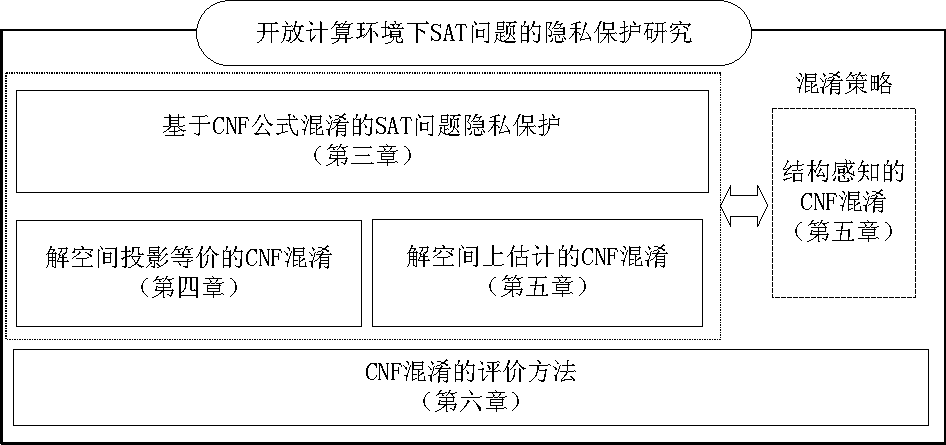
\includegraphics[width=0.8\textwidth]{fig103}
  \caption{本文研究内容}
  \label{fig:103}
\end{figure}

本文受国家高技术研究和发展计划“智能云服务与管理平台核心软件及系统”(项目编号2013AA01A212)和国家自然科学基金项目“面向通讯应用的自动对偶综合研究”(项目编号61070132)的支持,主要贡献和创新点如下:

1. 开放环境下基于加噪CNF混淆的SAT求解框架。
CNF公式混淆是保证开放环境下的SAT求解隐私性的重要手段。现有的方法基于双射或多射群加密,通过分段坡度编码对CNF 公式进行混淆,从而隐藏CNF公式中携带的结构信息。
但是这种方法改变了原有CNF公式的外部表示,需要设计新的求解算法。
并且在目前仅可使用全空间遍历的方法进行求解,无法利用已有成熟的SAT 求解算法,因此极大降低了其实用性。
本文通过对CNF公式自身逻辑特点的分析,提出了基于加噪思路的混淆算法。通过在原始CNF公式中无缝的混入噪音公式,在隐藏原有的结构信息的同时,保持原有的CNF 数据形式和解空间,从而复用目前已有的求解算法。
这就在算法的实用性和隐私保护上取得了良好的折中。
本文从理论上证明了算法的正确性并通过大量的仿真实验验证了算法的性能。

2. 解空间上估计的CNF混淆算法。
由于SAT求解时,输出数据也包含了敏感信息。
在研究了隐藏结构信息的CNF混淆算法之后,本文进一步研究了隐藏CNF 解的混淆方法。针对输出信息保护,本文提出了解空间上估计的CNF混淆算法。
通过扩展噪音公式解空间,使得混淆后SAT问题的解空间为原始解空间的上估计。
通过引入噪音解实现对原始解的隐藏。
本文从理论上充分证明了算法的正确性,并通过大量的仿真实验验证了方法的有效性和性能。

3. 混淆后公式的求解效率是在混淆算法有效性的一个特别重要的指标,也是基于加噪的混淆算法区别于其他混淆算法的一个重要因素。
由于加噪的过程改变了公式的内在结构,并且SAT问题自身特点,使得其问题复杂度会随着结构的变化出现跃变。
针对这一情况,本文针对硬件验证中常用的CNF结构进行分析,提出了跃变敏感的混淆策略,使得混淆后的CNF公式求解难度不会大于原始公式求解难度。
特别针对对偶综合这一SAT问题的实例算法进行了分析。从理论上验证了算法的可用性。

4. CNF混淆算法的有效性评价。
混淆算法保证混淆后的CNF公式可用已有的求解器求解,并且可以用较小的开销恢复出原始的解。
但是除此之外,在开放环境下为保证SAT 计算外包的顺利实施,混淆算法仍然需要满足其他的特性。
结合程序混淆的有效性评价标准,本文抽象出CNF公式混淆的有效性评价标准。
通过对混淆策略的细分,针对两种混淆策略进行定量分析和定性评价,为设计出更好的混淆策略提供了依据。

上述各部分研究内容之间的关系参见图1.3。
\section{论文组织结构}
论文共分六章,组织结构如下:
%TO DO 论文共分七章,组织结构如下:

第一章为绪论,介绍SAT求解的基本概念、特点、应用以及安全可验证计算的研究现状。分析CNF公式混淆算法的研究意义和挑战,并简述本文的研究内容和组织结构;

第二章为相关研究,对科学计算外包隐私保护、安全可验证计算以及程序混淆等相关概念进行了系统和全面的介绍,分析了现有工作的特点和适用性;

第三章研究SAT问题求解中输入数据的隐私保护问题,从实用性的角度出发,提出了基于加噪的CNF混淆算法。
在保证求解算法和解空间不变的前提下,通过混入噪音变量和子句来实现CNF公式内部结构信息的隐藏;

第四章在前述开创性工作的基础上,针对高危险外包计算环境,针对可能出现的ALLSAT攻击,通过引入具有簇形解的噪声CNF 公式,进一步提高混淆算法的鲁棒性;

第五章研究SAT问题求解中输出数据的隐私保护问题,提出了解空间上估计的CNF混淆方法,通过混入用户可剔除的噪声解来隐藏真实的解信息;
另一方面,研究SAT问题求解中输入数据中结构信息的增强型隐藏方法,提出在感知原有公式结构的基础之上,加入可构成合法结构的噪声变量和子句,来实现CNF公式内部结构的保真隐藏,以提高应对基于模式识别和同构检测等隐私攻击的防范能力;

%%第六章研究相变敏感的混淆算法,希望对混淆后的CNF公式求解效率进行有效控制。
第六章研究SAT问题混淆算法的有效性评价问题,希望通过对有效性标准的提取,为设计更为有效的混淆算法提供指导。
%
%第七章总结全文并展望未来的工作。

第七章总结全文并展望未来的工作。
最后是致谢、博士期间撰写的论文、参加的科研工作以及参考文献。
